\documentclass{scrreprt}

% allow images
\usepackage{graphicx}
% allow chinese
\usepackage{CJK}
% lists
\usepackage{enumitem}
% hyperlinked TOC (note the CJKbookmarks boolean)
\usepackage[CJKbookmarks = true]{hyperref}
% allow figures and tables to hold position
\usepackage{float}
% pretty tables
\usepackage{booktabs}
\usepackage[table]{xcolor}
% symbols
\usepackage{gensymb}
% format headers and footers
\usepackage[automark,headsepline,footsepline,plainfootsepline]{scrlayer-scrpage}
% allow for usage of \Blinddocument to test formatting
\usepackage{mwe}
% import tables from CSV files
\usepackage{csvsimple}

% options
\graphicspath{{./figures/} {../}}
\definecolor{light-gray}{gray}{0.95}
%% alternate table row colors
\rowcolors{1}{white}{light-gray}

% define macros
\newcommand{\pchapter}[1]{
	\begingroup\let\clearpage\relax
	\newpage
	\begin{figure}[H]
		
\includegraphics[width=0.25\textwidth]{logo.jpeg}
	\end{figure}
	\chapter{#1}
	\endgroup
}
\newcommand{\modelno}{%
	\texttt{FLT-A100}
}
\newcommand{\upstream}{
	\small\texttt{https://github.com/diracs-delta/fruition-specs/%
		      tree/master/FLT-A100-EN}
}
\newcommand{\x}{
	$\times$
}
\newcommand{\ptable}[2]{
	\begin{table}[H]
	\caption{#2}
	\centering\csvautobooktabular{#1}
	\end{table}
}

% define header, title, date
\lohead{
\includegraphics[width=\marginparwidth]{logo.jpeg}}
\title{
	\begin{figure}[H]
		\centering
\includegraphics[width=0.5\textwidth]{logo.jpeg}
	\end{figure}
	\vspace{1cm}
	\flushright
	\Huge{IMU MODULE}\\
	\Huge{HARDWARE SPECIFICATION}\\
	\vspace{2cm}
	\huge{Model No. \modelno}\\
	\vspace{2cm}
	\LARGE{Prepared by David Qiu \\ on behalf of FRUITION CO., LTD.}
}
\date{
	Last revision: January 11th, 2019\\
	\vspace{0.5cm}
	Full revision history and latest data sheets are available at\\
	\vspace{0.25cm}
	\upstream.
}
%%%%%%%%%%%%%%%%%%%%%%%%%%%%%%%%%%%%%%%%%%%%%%%%%%%%%%%%%%%%%%%%%%%%%%%%%%%%%%%%
\begin{document}
\begin{CJK*}{UTF8}{gbsn}
\maketitle
\tableofcontents

\pchapter{Product Overview}
\section{General Description}
The \modelno is Fruition's latest inertial measurement unit (IMU) module, an
economical solution to any hardware application in need of gyroscopic or
accelerometric measurements.

The \modelno IMU module is a tri-axis accelerometer and gyroscope, integrated
with an energy-efficient microprocessor suitable for low power applications. The
module firmware also contains an advanced signal processing algorithm aimed at
noise reduction. It also contains a sensor fusion algorithm that outputs its
three principal axes, i.e.\ its roll, pitch, and yaw. The module also supports
UART communication through its stamp half-hole patch interface.

Our module is especially suitable towards robotics industries necessitating
modules that are space-efficient. The \modelno IMU module is only
15.2\x17.8 mm in size, making it perfect for such applications.

\section{Features}
\begin{itemize}
\item Small size that is competitive with existing MEMS sensors.

\item Integrated high-precision six-axis gyroscope.

\item UART interface with high baud rate and I/O frequency.

\item Accurate sensor fusion algorithm that calculates the roll, pitch, and yaw.

\item High stability against thermal and vibrational fluctuation.

\item Low power consumption.
\end{itemize}

\section{Applications}
\begin{itemize}
\item Inertial navigation system for all portable robots, such as flying drones,
autonomous lawn mowers, or robot vacuums.
\end{itemize}

\section{Module Dimensions}
\begin{figure}[H]
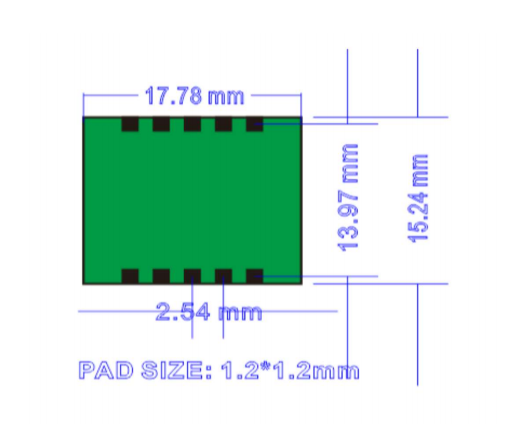
\includegraphics{module_dim.png}
\caption{General dimensions of the \modelno IMU module.}
\end{figure}

\section{Operating Ranges}
\begin{itemize}
\item Operating temperature range: $-40$/$+85$ \degree C
	\begin{itemize}
	\item Recommended: $-20$/$+70$ \degree C.
	\end{itemize}

\item Storage temperature range: $-40$/$+125$ \degree C.

\item Maximum working voltage (GND/VCC): $-0.3$V/$+4.5$V.
	\begin{itemize}
	\item Recommended: $-0.15$V/$3.3$V
	\end{itemize}

\item Maximum acceleration: $\pm$40 m/s$^2$ along any axis.

\item Maximum angular velocity: $\pm$1000 degrees/second (dps) along any axis.

\item Maximum pitch and roll: $\pm$ 90 degrees.

\item Maximum yaw: $\pm$ 180 degrees.
\end{itemize}

\section{Coordinate System Reference}
The most sensitive axis of the \modelno IMU module is perpendicular to the
module's plane. This is labelled the Z axis. The roll, pitch, and yaw are all
defined using the right-hand-rule, and are defined to be in the direction of
rotation with respect to the X, Y, and Z axes, respectively.

\pchapter{Module I/O}
\section{General I/O Scheme}
\begin{figure}[H]
\caption{Flowchart depicting the I/O scheme of the \modelno IMU module.}
\centering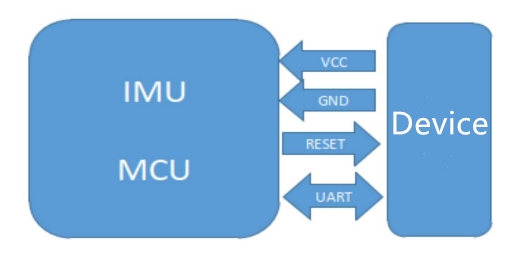
\includegraphics{module_io}
\end{figure}

\begin{figure}[H]
\caption{Location of pins on the \modelno IMU module}
\centering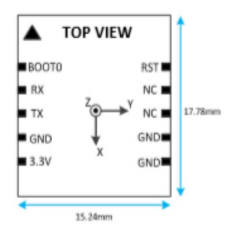
\includegraphics{module_top}
\end{figure}

\begin{figure}[H]
\caption{Circuit diagram of the \modelno IMU module}
\centering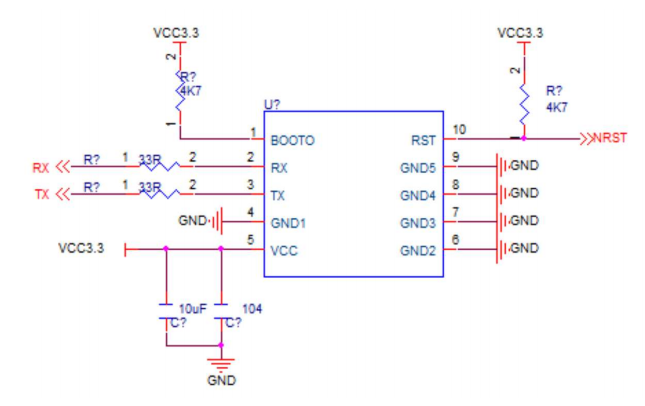
\includegraphics{circuit_diagram}
\end{figure}

\section{Pin Definitions}
\ptable{tables/pin_definitions.csv}{Pin definitions of the \modelno IMU module.}

\section{Communication Protocol}
The \modelno IMU module utilizes the UART communication interface, configured as
follows.

\begin{itemize}
\item Baud rate: 115200.

\item 8-bit data length.

\item No odd/even verification.

\item 1-bit stop.
\end{itemize}

The \modelno IMU module provides outputs data at 100 packets/second (Hz). The
format of each data packet is as follows.

\ptable{tables/packet_breakdown.csv}{%
	Breakdown of the data packets output by the \modelno IMU module. The
	units of the pitch, roll, yaw are in units of degrees. The units of the
	acceleration are in units of m/s$^2$. The units of angular velocity are
	in dps. The units of temperature are in \degree C.
}

An example data packet may appear as the following.

\begin{verbatim}
0xFF FE 00 5E 05 02 00 5D26 34 01 4F 06 1E 0A 12 47F2 1A E4 B2 F4 00 00 89
\end{verbatim}

The breakdown of this example packet is as follows.

\ptable{tables/packet_example.csv}{%
	Interpretation of the above example data packet.
}

\subsection{Status Byte Interpretation}

The status byte has three possible values.

\begin{itemize}
\item \textbf{Status = 0}: IMU Calibration successful. The data contained within
this packet has the highest accuracy.

\item \textbf{Status = 1}: Excessive tilt detected during IMU calibration.
Please re-calibrate.

\item \textbf{Status = 2}: Excessive motion detected during IMU calibration.
Angular measurements remain accurate. Please re-calibrate.

\item \textbf{Status = 3}: Excessive tilt and excessive motion detected during
IMU calibration. Please re-calibrate.
\end{itemize}

\chapter{Supplementary Information}
\begin{figure}[H]
\centering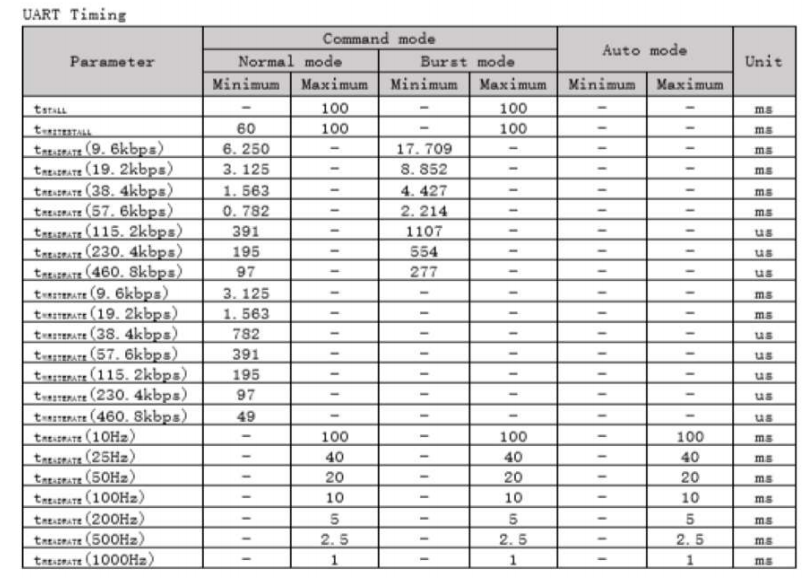
\includegraphics[width=\textwidth]{uart_timing}
\end{figure}

\pchapter{Legal}
\section{Safety Information}
This device is sensitive to electrostatic discharge (ESD). Though the module
comes with standard ESD circuit protection, the components may still malfunction
if ESD occurs. Standard ESD precautions should be taken when handling this
device.

\section{Liability}
\textbf{SHENZHEN FRUITION CO., LTD.} shall not be liable, under any
circumstances, for any special, indirect, incidental, consequential, or
contingent damages for any reason, whether or not the buyer has been advised of
the possibility of such damage.

\end{CJK*}
\end{document}
%%%%%%%%%%%%%%%%%%%%%%%%%%%%%%%%%%%%%%%%%%%%%%%%%%%%%%%%%%%%%%%%%%%%%%%%%%%%%%%%
